\section{Siamese Neural Network (SNN)}
Siamese Neural Network (SNN), çift girişli bir sinir ağı mimarisidir. Benzerlik veya eşleştirme gibi problemleri çözmek için kullanılırlar. İki farklı örnek arasındaki benzerliği belirlemek için kullanılır. Siamese ağları birbirinin aynısı 2 veya daha fazla ağdan oluşur. Bu ağlar, her bir veri örneğini ayrı ayrı işler ve her biri için bir özellik vektörü üretir. Üretilen özellik vektörleri bir mesafe fonksiyonu kullanılarak karşılaştırılır. Model, tahminin olasılıklarını değil, her bir sınıfa olan mesafeyi verir. 

\begin{figure}[h]
    \centering
    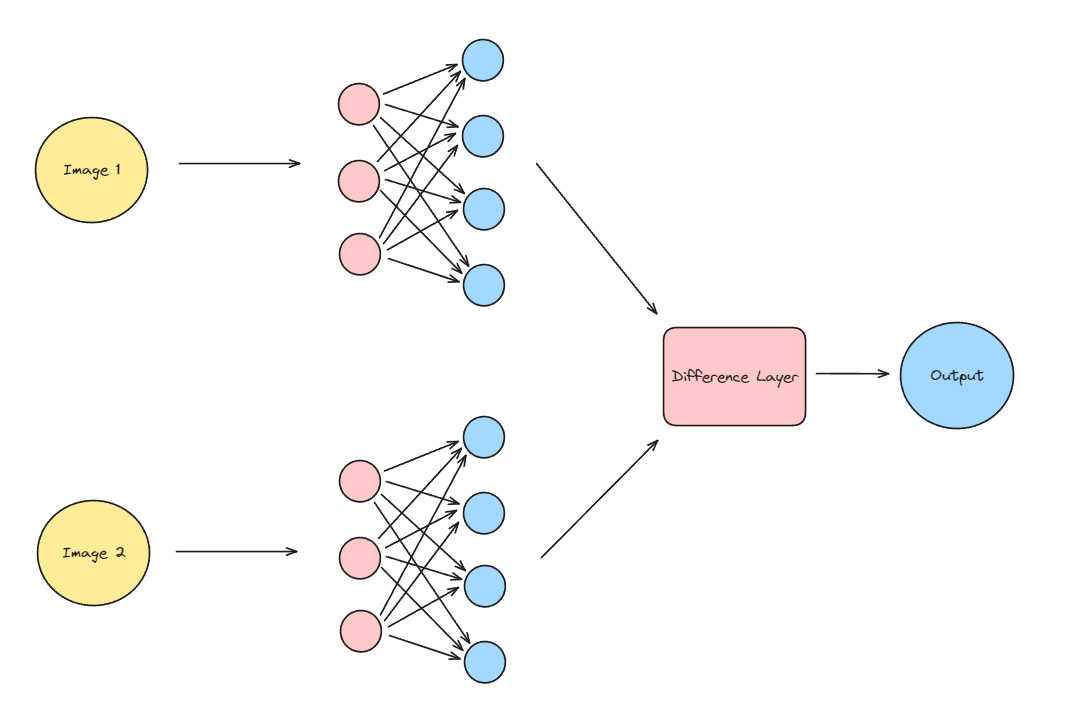
\includegraphics[width=1\textwidth]{images/siamese_neural_network.png}
    \caption{Siyam sinir ağı mimarisi.}
    \label{fig:enter-label}
\end{figure}

\subsection{Çalışma Adımları}
\begin{enumerate}
    \item Her bir örnek için özellik vektörü çıkarılır.
    \item Çıkarılan örnekler, bir mesafe fonksiyonu kullanılarak karşılaştırılır. Örneğin öklid mesafesii, kosinüs benzerliği, kontrastif kayıp fonksiyonu gibi.
    \item Bu karşılaştırma sonucunda bir çıktı üretilir.
\end{enumerate}

\newpage